\documentclass[12pt, a4paper, oneside]{ctexart}
\usepackage{fancyhdr}
\usepackage{amsmath, amsthm, amssymb, bm, graphicx, hyperref, mathrsfs, graphicx, float, subfigure, caption, makecell, longtable,framed}
\usepackage[dvipsnames]{xcolor}
\usepackage{listings}
\renewcommand{\lstlistingname}{代码清单}
\lstset{
    language=C++, % 设置语言
 basicstyle=\ttfamily, % 设置字体族
 breaklines=true, % 自动换行
 keywordstyle=\bfseries\color{NavyBlue}, % 设置关键字为粗体,颜色为 NavyBlue
 morekeywords={}, % 设置更多的关键字,用逗号分隔
 emph={self,input,output,wire,reg,posedge,negedge}, % 指定强调词,如果有多个,用逗号隔开
    emphstyle=\bfseries\color{Rhodamine}, % 强调词样式设置
    commentstyle=\itshape\color{black!50!white}, % 设置注释样式,斜体,浅灰色
    stringstyle=\bfseries\color{PineGreen!90!black}, % 设置字符串样式
    columns=flexible,
    numbers=left, % 显示行号在左边
    numbersep=2em, % 设置行号的具体位置
    numberstyle=\footnotesize, % 缩小行号
    frame=single, % 边框
    framesep=1em % 设置代码与边框的距离
}
\renewcommand\thesubsection{\zhnum{subsection}、}
\renewcommand\thesubsubsection{\arabic{subsubsection}.}
\renewcommand\theparagraph{(\arabic{paragraph})}
\renewcommand\thesection{}
\usepackage[left=1in, right=1in, top=1in, bottom=1in]{geometry}

\pagestyle{fancy}
\fancyhf{}
\renewcommand{\headrulewidth}{0pt}
\fancyfoot[C]{\thepage}

\title{\textbf{工科创II 心率检测算法实验报告}}
\author{张浩宇 522031910129}
\date{}

\begin{document}
    \maketitle
    \subsection{实验流程与代码}
    根据已有的PPG数据,通过不同的心率检测算法,得到心率数据,并与参考心率对比,比较不同的算法的效果.
    \subsubsection{峰值检测法}
    通过检测一段信号中的峰值数目来计算心率.基本原理是最大最小值法,即找到信号中满足值大于两边的位置,这些位置即为峰值.由峰值位置和个数即可计算心率.
    
    为了解决次波峰的影响,可采用阈值法,设定一定的阈值,只有超过阈值的峰才被记录.同时可利用滑动平均法处理信号,消除次波峰和毛刺.
    也可以根据人类心率范围和心率变化速度设定超参数限制,对偏差过大的数据进行处理.
    \subsubsection{数字滤波}
    PPG信号可看作是原始心率信号和其他各种噪声信号的叠加,若用滤波器对信号预处理,滤除噪声,留下较为纯净的心率信号来计算心率,可得到较为准确的结果.
    \subsubsection{频谱分析法}
    PPG是一种跟随心跳的伪周期信号,因此可以用频谱来分析心率. 快速傅里叶变换FFT可以快速求得PPG信号的频谱,在频谱中最高峰对应的频率就是心率信号的频率,由此可以计算出心率.
    同时也可引入超参数限制来优化结果.

    \subsection{结果分析}
    分别用不同算法对有噪声的PPG数据进行心率检测,将结果与参考心率对比,如图1所示.

    \begin{figure}[H]
        \centering
        \subfigure[简单噪声;峰值法]{
          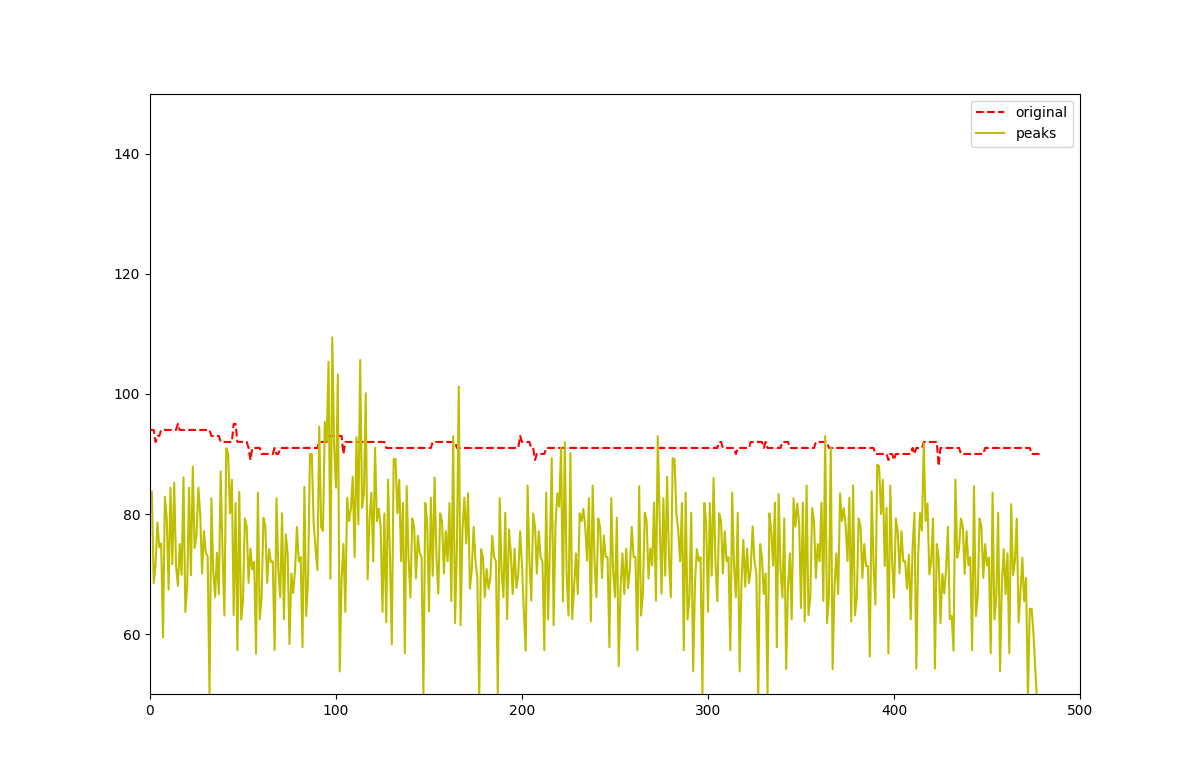
\includegraphics[width=0.4\textwidth]{img/peaks_noise.png}}
        \subfigure[复杂噪声;峰值法]{
          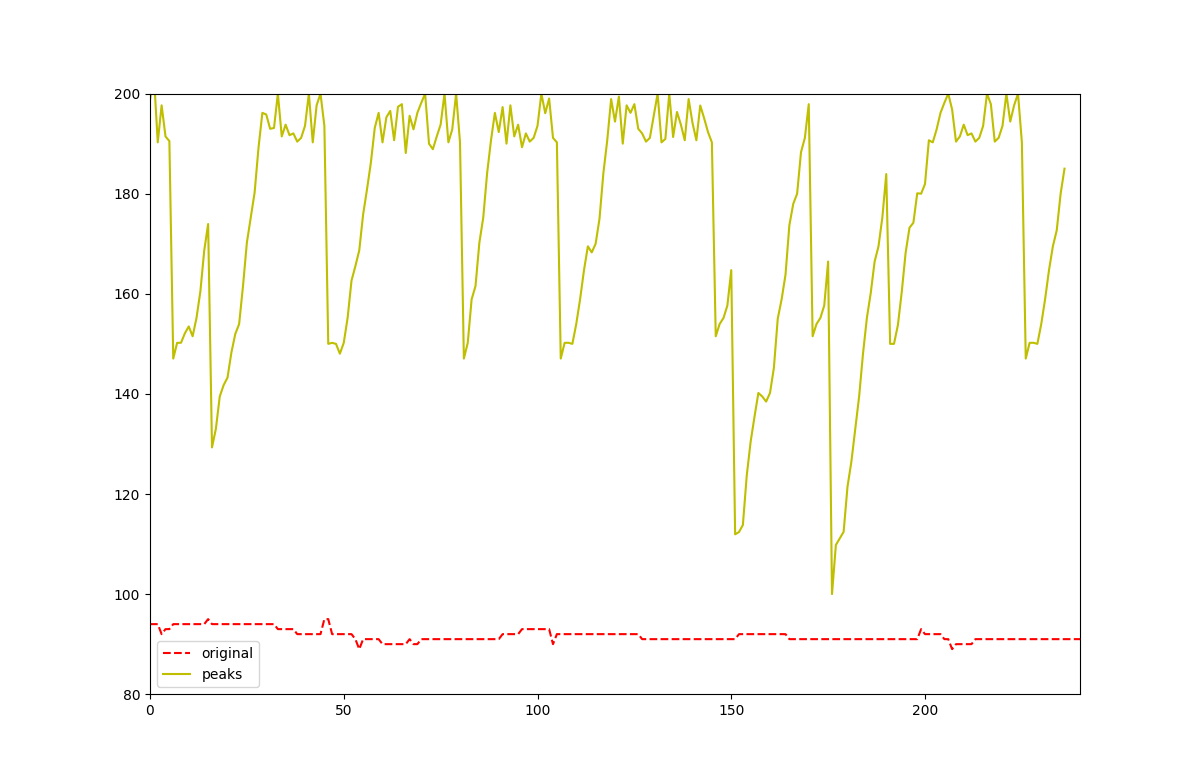
\includegraphics[width=0.4\textwidth]{img/peaks_ma.png}}
          \subfigure[简单噪声;滤波+峰值法]{
          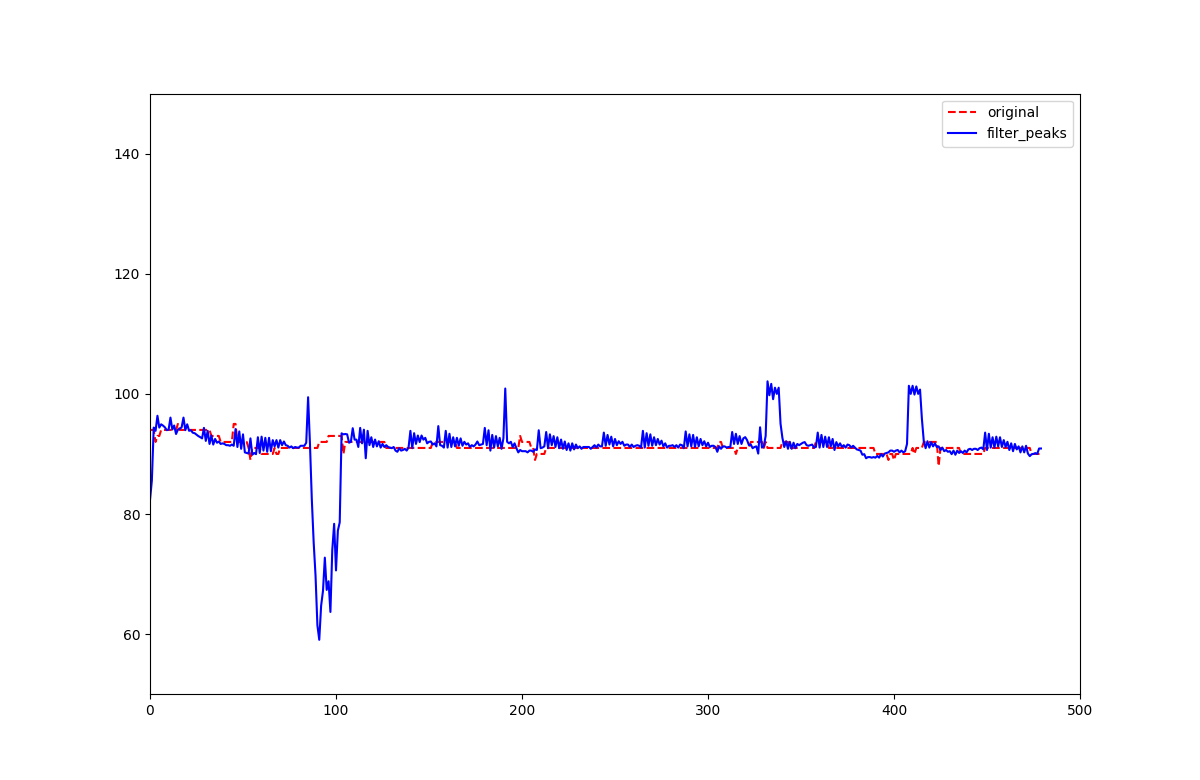
\includegraphics[width=0.4\textwidth]{img/filter_noise_1_890.png}}
          \subfigure[复杂噪声;滤波+峰值法]{
          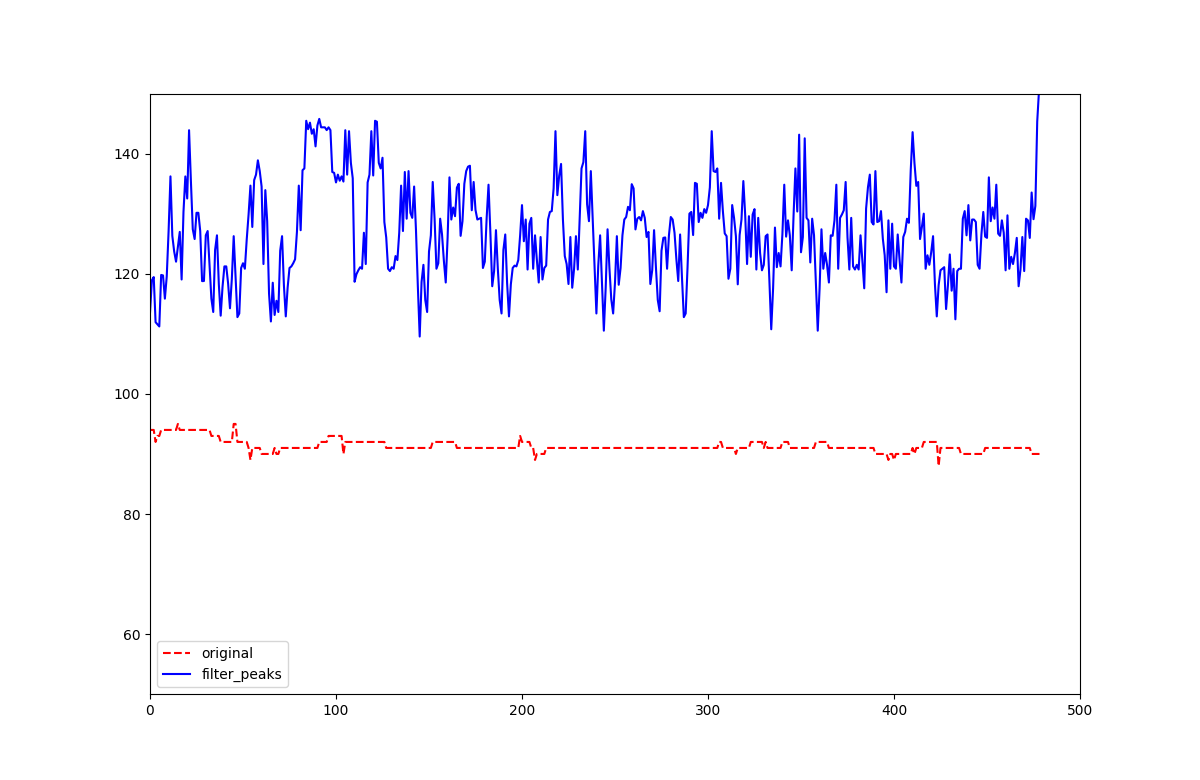
\includegraphics[width=0.4\textwidth]{img/filter_ma.png}}
          \subfigure[简单噪声;滤波+FFT]{
          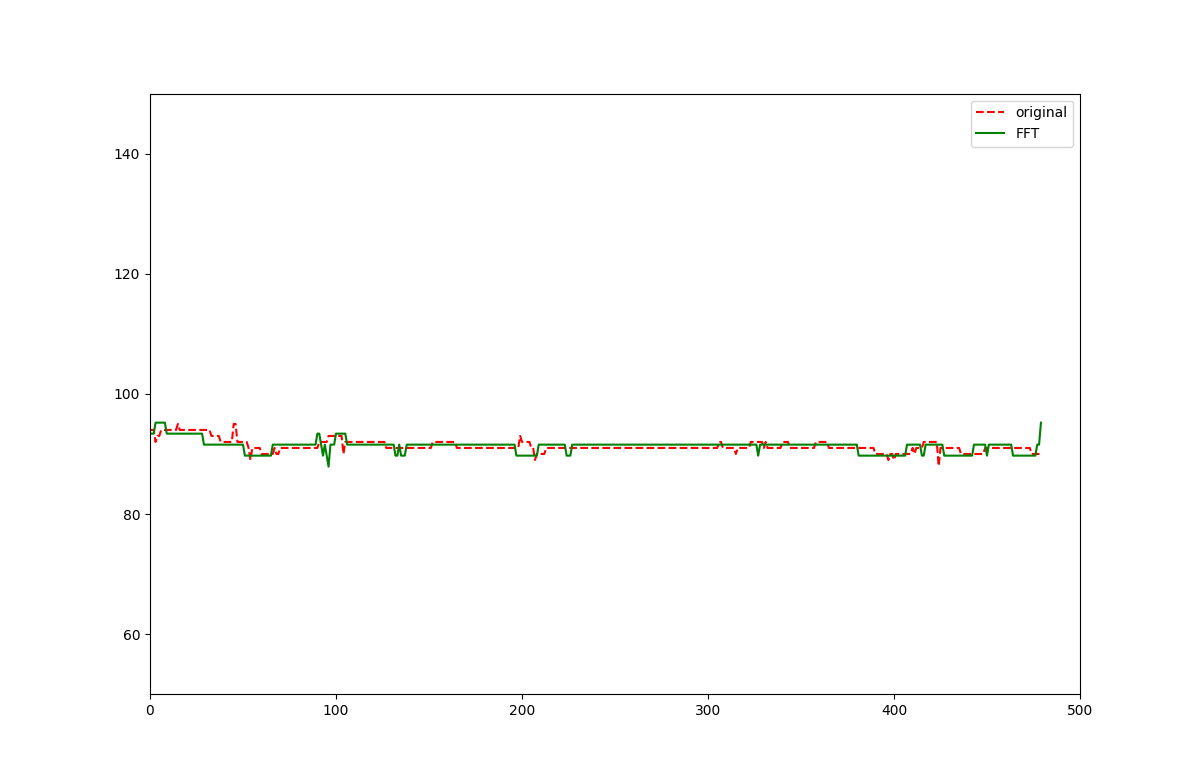
\includegraphics[width=0.4\textwidth]{img/ftt_noise_0_781.png}}
          \subfigure[复杂噪声;滤波+FFT]{
          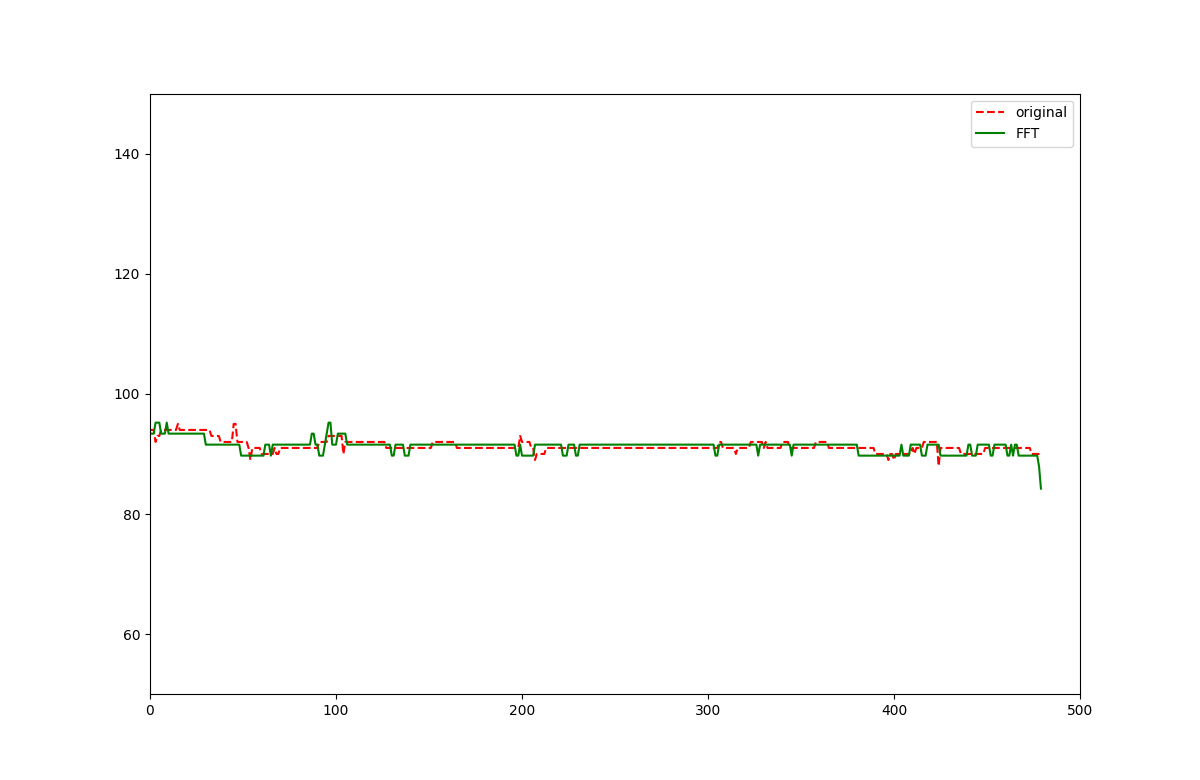
\includegraphics[width=0.4\textwidth]{img/ftt_ma_0_811.png}}
        \caption{心率检测结果与参考心率}
        \label{fig:twopicture} 
      \end{figure}

      根据图1(a)(c)(e),当信号有简单的高低频噪声时,单独的峰值法已经有较大偏差;经过滤波后的峰值法也有一定的偏差,且波动较大,
      经计算平均误差1.890;而滤波后使用频谱法效果较好,偏差很小,且比较稳定,经计算平均误差0.781.

      根据图1(b)(d)(f),当信号带有复杂的噪声和伪影时,峰值法和经过滤波的峰值法结果均偏差较大,而滤波后使用频谱法效果较好,偏差较小,
      经计算平均误差0.811.

      因此经过滤波的FFT频谱法效果相比峰值法更好.因为峰值法只关注局部是否出现峰值,很易受噪声影响;而频谱法与信号整体特征有关,且可将不同频率成分分开,
      可以减少噪声的影响,经过滤波可以进一步消除噪声,从而得到比较好的检测效果.



\end{document}

